\subsection{Methodological Literature}

Based on the systematic review and its coding, the first data set we
assess is a database of scale validations. We bring together the scales
suggested in previous reviews as well as validation studies we
identified in our own review. Throughout our literature review we found
five major works that reviewed the measurement of acculturation
\citep{Celenk2011, Maestas2000, Matsudaira2006, Wallace2010, Zane2004}.
After the removal of duplicate scales, we added any scale validation
that was present in our own systematic review but not included in the
previous reviews. For each measure we extracted the full item list as
well as the item scoring prior to coding. A comprehensive and
interactive database of the scales, with reference- and publication
information, as well as our experience elements and -context coding is
available in our online supplementary information as well as on our open
science repository (OSF and/or github citation here).

\subsubsection{Methods}

Taken together these five reviews collected a total of 197 scales, of
which 75 were duplicates. From our own review we added 25 additional
validation studies. After removing duplicates this meant that we
considered a total of 122 unique scales for our coding. Of these scales
we ultimately had to exclude 41, because they were either not accessible
or did not fit the the topic of our review (see Table
\ref{tab:ScalesExclusion}). The scales had an average of \hl{X.XX} items
and \hl{X.XX} sub-scales. Most items were rated on a five-point
(\hl{XX.XX}\%) or four-point likert-type scale (\hl{XX.XX}\%), with only
\hl{X} scales including categorical ratings. About a fifth of scales
(20.4918\%) included majority group members in their validation studies.
The earliest included validation was from 1972 with a majority of scales
being validated around the turn of the 21\textsuperscript{st} century
and the latest included validation study in 2018.

\begin{table}

\caption{(\#tab:ScalesExclusion)Reasons for Exclusion}
\begin{tabular}[t]{lc}
\toprule
Exclusion Reason & Frequency\\
\midrule
not migration & 14\\
items not included & 8\\
search pending & 5\\
not accessible & 4\\
not found & 3\\
not acculturation & 2\\
majority focussed & 1\\
not found probably the same as Tsai et al. 2000 & 1\\
only language (no scale) & 1\\
same as S-029 & 1\\
uses other scale & 1\\
\bottomrule
\end{tabular}
\end{table}


\subsubsection{Results}

For the literature on scale validations, we assessed both the role of
experience elements in the measures as well as contextual differences.

\paragraph{Experience}

With our main aim of examining the experience structure within the
scales, we examined whether scales included a specific experience
elements but also examined the used elements in their complex
combinations. In terms of general inclusion of elements, most studies
included a measure of cognition (89.66\%) and behavior (82.76\%),
whereas only roughly half the studies included a measure of affect
(55.17\%) and only a fourth of the scales included a measure of motives
(28.74\%). However, only a minority of scales included only a single
dimension. There were only 5 scales that exclusively relied on
cognitions (5.75\%) and 4 scales that measured only behaviors (4.6\%).
Yet, inversely, there were also only 13 scales that measured all four
dimensions (14.94\%). Most studies measured two (37.93\%) or three
(36.78\%) dimensions. A majority of scales either measured behavioral
and cognitive elements (26.44\%) or behavioral, cognitive, and affective
elements (26.44\%; also see Figure \ref{fig:ElementsScales}). Looking at
the number of elements measured together we also see substantial
differences in what kind of scales include a certain element. Scales
that included cognitions measured an average of 2.67 elements, scales
measuring behavior, on average, measured a 2.71, while scales that
included affect measures had a complexity average of 3.1 and scales
measuring motivation even measured an average of 3.4 scales. Thus, most
scales measure multiple dimensions, yet they focus on easily accessible
dimensions (i.e., behavior and cognition), less of what is considered
`less accessible' or `subjective' (i.e., affect and desires). This is
also visible in the circumstance that there were no scales that
exclusively measured motivational or emotional adaptation (while this
was the case for both cognitions and behaviors). And if emotional or
motivational aspects were measured they were on average measured in
scales that were already more complex (i.e., included more experience
elements).

\begin{figure}[h]
\centering
\caption{Bar graph of the experience element combinations.}
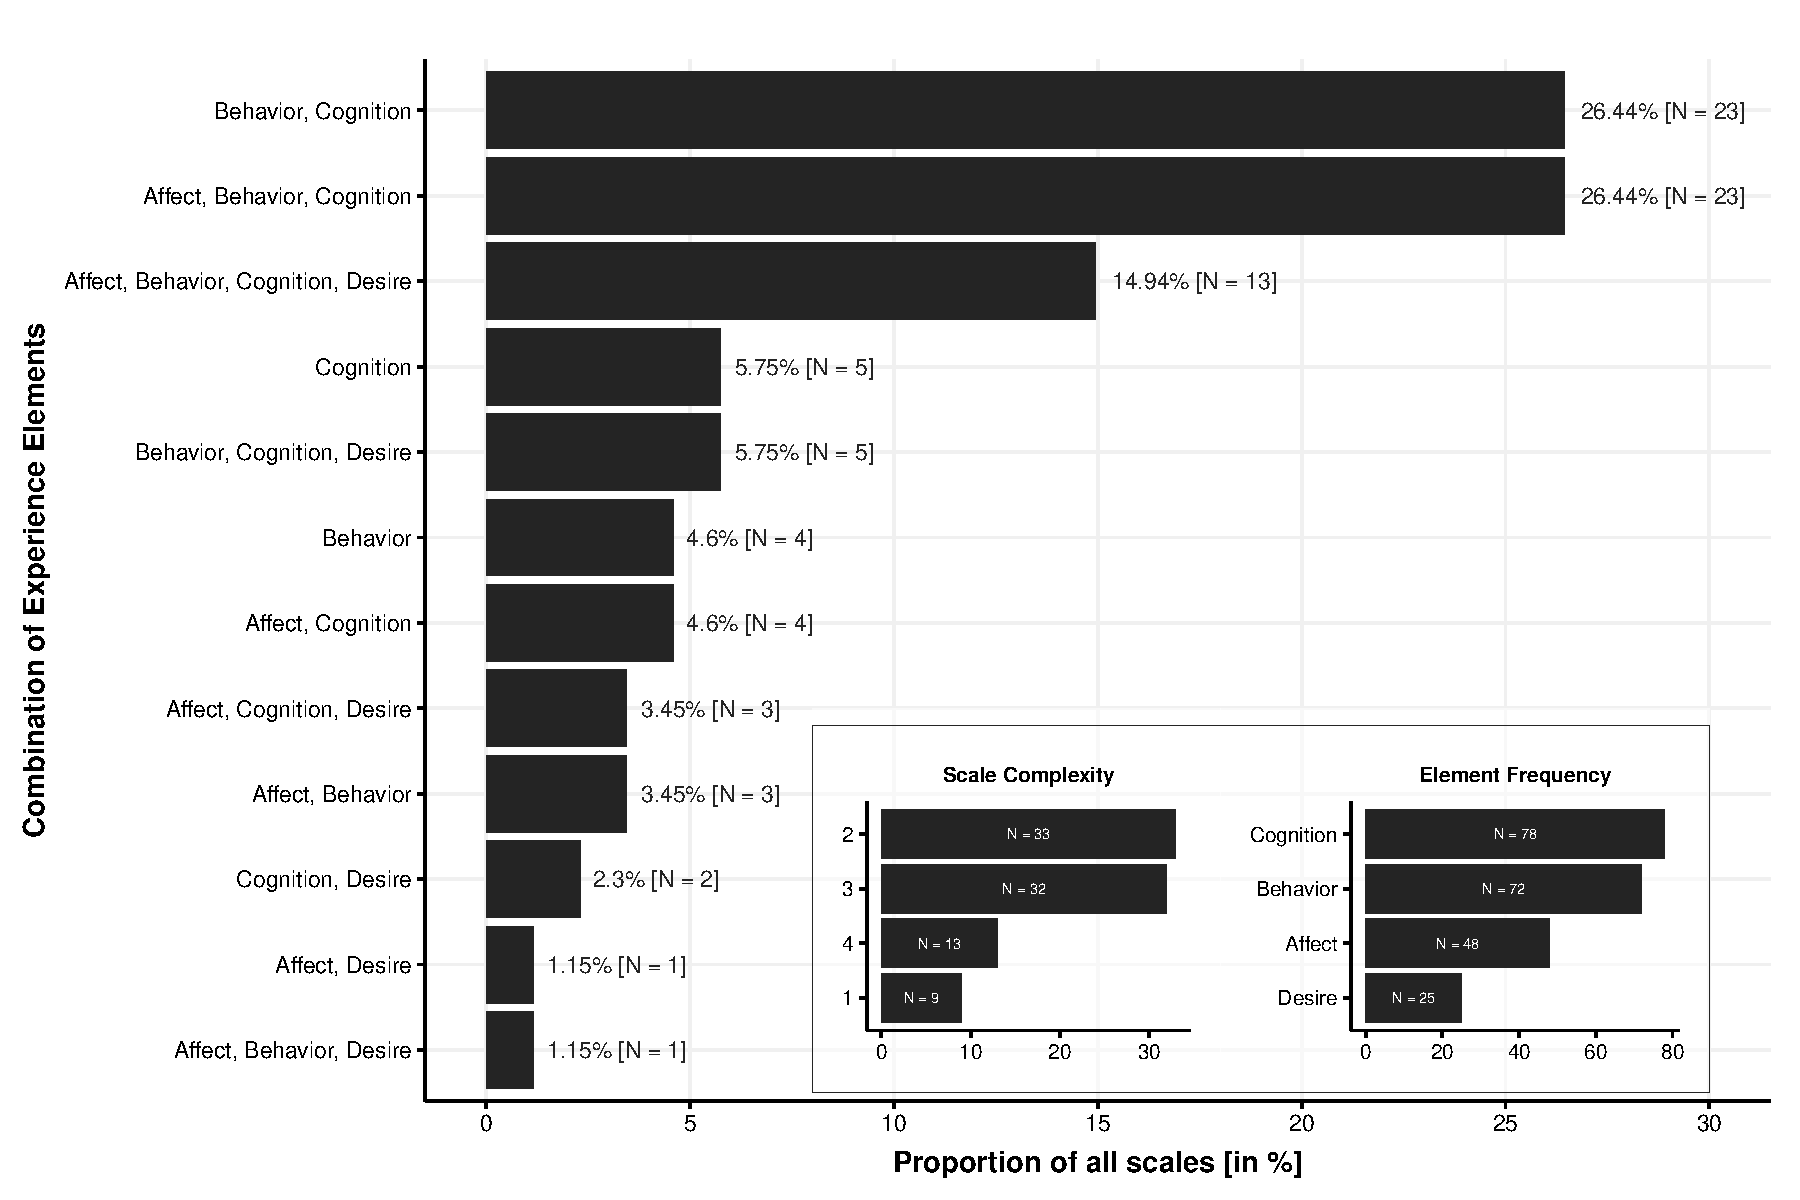
\includegraphics[width=\textwidth]{Figures/ABCDFreq-1}
\label{fig:ElementsScales}
\end{figure}

END SECTION
